\documentclass[12pt,a4paper,bibliography=totoc,listof=totoc]{scrartcl}
% u.U. muss Koma-Skript Package ueber MikTeX deinstalliert und neu installiert werden
% Hilft das nicht, so sollte statt scrartcl die Dokumentenklasse article verwendet werden
\usepackage[ngerman]{babel}
\usepackage[utf8]{inputenc}
\usepackage{ifthen}
\usepackage{xargs}
\usepackage{amsmath}
\usepackage{amsfonts}
\usepackage{amssymb}
\usepackage{graphicx}
\usepackage{fancyhdr}
\usepackage{tabularx}
\usepackage{geometry}
\usepackage{setspace}
\usepackage[right]{eurosym}
\usepackage[printonlyused]{acronym}
\usepackage{subfig}
\usepackage{floatflt}
\usepackage{float}
\usepackage[usenames,dvipsnames]{color}
\usepackage{colortbl}
\usepackage{paralist}
\usepackage{array}
\usepackage{parskip}
\usepackage[right]{eurosym}
\usepackage[subfigure,titles]{tocloft}
\usepackage[pdfpagelabels=true]{hyperref}

\usepackage{listings}
\lstset{basicstyle=\footnotesize, captionpos=b, breaklines=true, showstringspaces=false, tabsize=2, frame=lines, numbers=left, numberstyle=\tiny, xleftmargin=2em, framexleftmargin=2em}
\makeatletter
\def\l@lstlisting#1#2{\@dottedtocline{1}{0em}{1em}{\hspace{1,5em} Lst. #1}{#2}}
\makeatother

\geometry{a4paper, top=35mm, left=35mm, right=25mm, bottom=40mm, headsep=10mm, footskip=10mm}

\definecolor{codered}{rgb}{0.6,0,0} % for strings
\definecolor{codegreen}{rgb}{0.25,0.5,0.35} % comments
\definecolor{codepurple}{rgb}{0.5,0,0.35} % keywords
\definecolor{codeblue}{rgb}{0.25,0.35,0.75} 
\definecolor{codegray}{rgb}{0.6,0.6,0.6}
 
\lstset{language=C,
basicstyle=\ttfamily\footnotesize,
keywordstyle=\color{codepurple}\bfseries,
stringstyle=\color{codered},
commentstyle=\color{codegreen}\itshape\bfseries,
morecomment=[s][\color{codeblue}]{/**}{*/},
numbers=left,
numberstyle=\tiny\color{codegray},
stepnumber=1,
numbersep=10pt,
tabsize=2,
showspaces=false,
showstringspaces=false}


% begin change
%\titlespacing{\section}{0pt}{12pt plus 4pt minus 2pt}{-6pt plus 2pt minus 2pt}
% end change

% Kopf- und Fusszeile
\renewcommand{\sectionmark}[1]{\markright{#1}}
\renewcommand{\leftmark}{\rightmark}
\pagestyle{fancy}
\lhead{}
\chead{}
\rhead{\thesection\space\contentsname}
\lfoot{}
\cfoot{}
\rfoot{\ \linebreak \thepage}
\renewcommand{\headrulewidth}{0.4pt}
\renewcommand{\footrulewidth}{0.4pt}

% Vorspann
\renewcommand{\thesection}{\Roman{section}}
\renewcommand{\theHsection}{\Roman{section}}
\pagenumbering{Roman}

\newcommand{\folgen}[1]{
\ensuremath
#1
}

\newcommandx{\student}[3][]{
	\def\studentName{#1}%
	\def\studentMatnr{#2}%
	\def\studentStudiengang{#3}%
}

\newcommandx{\studentt}[3][]{
	\def\studentNamet{#1}%
	\def\studentMatnrt{#2}%
	\def\studentStudiengangt{#3}%
}


\newcommandx{\studenttt}[3][]{
	\def\studentNamett{#1}%
	\def\studentMatnrtt{#2}%
	\def\studentStudiengangtt{#3}%
}
\newcommandx{\studentttt}[3][]{
	\def\studentNamettt{#1}%
	\def\studentMatnrttt{#2}%
	\def\studentStudiengangttt{#3}%
}
\newcommandx{\studenttttt}[3][]{
	\def\studentNametttt{#1}%
	\def\studentMatnrtttt{#2}%
	\def\studentStudiengangtttt{#3}%
}


\newcommandx{\MyTitelseite}[8][]{
\thispagestyle{empty}
%
\includegraphics[scale=0.2]{pics/oth-logo.png}\hfill\includegraphics[scale=0.2]{#1}

\includegraphics[scale=0.2]{pics/oth-logo.png}
\begin{center}
\ifthenelse{\equal{#2}{2}}{ % then
	\vspace*{2cm}
	\Large
	\textbf{Ostbayerische Technische Hochschule Regensburg}\\
	\textbf{Fakultät für Informatik und Mathematik}\\
	\vspace*{2cm}
	\Huge
	\textbf{#3}\\[1em]
	\large
	%Zur Erlangung des akademischen Grades des\\
	%\ifthenelse{\equal{#3}{Bachelorarbeit}}{Bachelor of Science (B.Sc.)}{Master of Science (M.Sc.)}\\
	\vspace*{1cm}
	\Large
	\textbf{#4}\\
}{ % else
	\vspace*{1cm}
	\Large
	\textbf{#4}\\
	\vspace*{2cm}
	\large
	An der Fakultät für Informatik und Mathematik der\\
	Ostbayerischen Technischen Hochschule Regensburg\\
	im Studiengang\\
	\studentStudiengang\\[2em]
	eingereichte\\
	\vspace*{1cm}
	\Large
	\textbf{#3}\\[2em]
	\large
	%zur Erlangung des akademischen Grades des\\
	%\ifthenelse{\equal{#3}{Bachelorarbeit}}{Bachelor of Science (B.Sc.)}{Master of Science (M.Sc.)}
	\vspace*{1cm}
	\Large
}
	\vfill
	\normalsize
	%\newcolumntype{x}[1]{>{\raggedleft\arraybackslash\hspace{0pt}}p{#1}}
	\begin{tabular}{rl}%{6cm}p{7.5cm}}
	    \rule{0mm}{1ex}\textbf{Name:} & \studentName \\
		\rule{0mm}{1ex}\textbf{Matrikelnummer:} & \hspace*{-0.5em}\begin{tabular}[t]{r}\studentMatnr\end{tabular} \\ 
		\rule{0mm}{1ex}\textbf{Name:} & \studentNamet \\
		\rule{0mm}{1ex}\textbf{Matrikelnummer:} & \hspace*{-0.5em}\begin{tabular}[t]{r}\studentMatnrt\end{tabular} \\ 
		\rule{0mm}{1ex}\textbf{Name:} & \studentNamett \\
		\rule{0mm}{1ex}\textbf{Matrikelnummer:} & \hspace*{-0.5em}\begin{tabular}[t]{r}\studentMatnrtt\end{tabular} \\ 
				\rule{0mm}{1ex}\textbf{Name:} & \studentNamettt \\
		\rule{0mm}{1ex}\textbf{Matrikelnummer:} & \hspace*{-0.5em}\begin{tabular}[t]{r}\studentMatnrttt\end{tabular} \\ 
				\rule{0mm}{1ex}\textbf{Name:} & \studentNametttt \\
		\rule{0mm}{1ex}\textbf{Matrikelnummer:} & \hspace*{-0.5em}\begin{tabular}[t]{r}\studentMatnrtttt\end{tabular} \\ 
		%\ifthenelse{\equal{#2}{1}}{~\\}{\rule{0mm}{1ex}\textbf{Studiengang:} & \studentStudiengang \\[2em]}
		\newline \\
		\rule{0mm}{1ex}\textbf{Erstgutachter:} & #5 \\ 
		\rule{0mm}{1ex}\textbf{Zweitgutachter:} & #6 \\[2em]
		\rule{0mm}{1ex}\textbf{Abgabedatum:} & #7 \\
	\end{tabular} 
	

%\end{center}	
%\end{center}
	
	
\end{center}
\pagebreak
}
\usepackage[utf8]{inputenc}
\usepackage[ngerman]{babel}
\begin{document}


% ----------------------------------------------------------------------------------------------------------
% Titelseite
% ----------------------------------------------------------------------------------------------------------
\student{Michael Braun}	% Studierender
{3113161}						% Matrikelnummer
{Technische Informatik}			% Studiengang

\studentt{Korbinian Federholzner}	% Studierender
{3114621}						% Matrikelnummer
{Technische Informatik}			% Studiengang

\studenttt{Philipp Kramer}	% Studierender
{1234456}						% Matrikelnummer
{Technische Informatik}			% Studiengang

\studentttt{Patrick Lesch}	% Studierender
{12344556}						% Matrikelnummer
{Technische Informatik}			% Studiengang

\studenttttt{Michael Schmidt}	% Studierender
{2907322}						% Matrikelnummer
{Technische Informatik}			% Studiengang


%\MyTitelseite{pics/oth-logo-informatik.png}	% Optionales Logo des extern betreuenden Unternehmens
\MyTitelseite{}
{1}								% Style der Titelseite (1 oder 2)
{Projektdokumentation (Datenverarbeitung in der Technik)}			% Typ der Arbeit 
{Balancing Plate}				% Thema der Arbeit						
{Prof.\ Dr.\ Richard Roth}   % Betreuer
{ Hr.\ Matthias Altmann}	% Zweitgutachter
{10.2.\the\year}				% Abgabedatum

\setcounter{page}{1} 

%-----------------------------------------------------------------------------------------------------------
% Abstract Zusammenfassung
%-----------------------------------------------------------------------------------------------------------
%\section*{Kurzfassung}
%...
%\pagebreak

%\section*{Abstract}
%...
%\pagebreak

%\section*{Danksagung}
%...
%\pagebreak

% ----------------------------------------------------------------------------------------------------------
% Inhaltsverzeichnis
% ----------------------------------------------------------------------------------------------------------
\tableofcontents
\pagebreak

% ----------------------------------------------------------------------------------------------------------
% Inhalt
% ----------------------------------------------------------------------------------------------------------
% Abstände Überschrift
% begin change
% alte Befehle
%\titlespacing{\section}{0pt}{12pt plus 4pt minus 2pt}{-6pt plus 2pt minus 2pt}
%\titlespacing{\subsection}{0pt}{12pt plus 4pt minus 2pt}{-6pt plus 2pt minus 2pt}
%\titlespacing{\subsubsection}{0pt}{12pt plus 4pt minus 2pt}{-6pt plus 2pt minus 2pt}
% neue Befehle
\RedeclareSectionCommands[
beforeskip=-.9\baselineskip,
afterskip=.4\baselineskip
]{section,subsection,subsubsection}
%end change

% Kopfzeile
\renewcommand{\sectionmark}[1]{\markright{#1}}
\renewcommand{\subsectionmark}[1]{}
\renewcommand{\subsubsectionmark}[1]{}
\lhead{Kapitel \thesection}
\rhead{\rightmark}

%\onehalfspacing
\setstretch{1.15}
\renewcommand{\thesection}{\arabic{section}}
\renewcommand{\theHsection}{\arabic{section}}
\setcounter{section}{0}
\pagenumbering{arabic}
\setcounter{page}{1}

% ----------------------------------------------------------------------------------
% Kapitel 1: Einleitung
% ----------------------------------------------------------------------------------
\section{Einführung/ Projektkontext}

%Grober Inhalt des Lastenhefts in Verbindung mit den Änderungen zur ersten Version (App als Pflicht, 
%keine Rückgabe der Servostellung). 
Der Grundaufbau des Prototyps ist eine Plexiglasplatte, auf der sich 
eine Kugel befindet. Diese Kugel wird durch Druck auf eine resistive Touch-Folie (Wertbestimmung durch 
Druck) erkannt und die zugehörigen Daten werden an einen Raspberry Pi 4 übermittelt. Dieser berechnet dann 
den Offset zum gewünschten Stellpunkt auf der Platte und mit Hilfe eines PID-Reglers die neuen Stellwerte 
für die Servomotoren. Diese Daten werden an einen XMC 4500 übermittelt, welcher die zuvor ermittelten Werte 
in PWM-Signale übersetzt und diese dann an die zuständigen Servomotoren übergibt. Diese bewegen die 
Plexiglasplatte, auf der sich die Touch-Folie befindet, um so die Kugel zu balancieren.
Die Versuchsapparatur soll selbstständig in der Lage sein eine Kugel auf einer Platte in eine vorher 
festgelegte Position, meist die Mitte der Platte, zu manövrieren. Dies soll durch Heben bzw. Senken der 
Plexiglasplatte mittels dreier Servomotoren geschehen. Optional ist dabei die manuelle Steuerung der 
Platte mittels einer App, welche über eine WiFi-Schnittstelle mit dem Raspberry Pi in Verbindung stehen 
soll. Diese App soll dabei das im Handy verbaute Gyroskop verwenden, um den Neigungswinkel des Geräts zu 
erfassen und die Platte dementsprechend zu neigen. Auch eine GUI sollte in der App vorhanden sein.
\newline Im Gegensatz zum Lastenheft, dass kurz nach dem Start abgegeben werden musste, haben sich im 
Laufe des Projektes einige Änderungen ergeben. Dabei wurde die Steuerung mittels einer iOS-App nunmehr 
als Pflichtmodul angesehen. Außerdem wurde das Auslesen der Potentiometer der Servomotoren aus Zeitgründen 
fallengelassen.
\pagebreak
% ----------------------------------------------------------------------------------
% Kapitel 2: Umsetzung
% ----------------------------------------------------------------------------------
\section {Umsetzung}
Um eine konsistente Abarbeitung zu gewährleisten wurde das Projekt in verschieden Module/Arbeitspakete 
geteilt.

\begin{tabularx}{\textwidth}{p{0.25\textwidth}|X|X|X|X|}
\hline
Name 					& Aufgabe 1 			& Aufgabe 2 				& Aufgabe 3  \\
\hline
Michael Braun			& Physischer Aufbau		& Reglerentwicklung			& PWM-Signale \\
\hline
Korbinian Federholzner	& Ansteuerung mit App	& UART Schnittstelle		& Touch-Folie \\
\hline
Philipp Kramer			&Reglerentwicklung		& Modellerstellung Matlab	& Touch-Folie\\
\hline
Patrick Lesch			& Ansteuerung mit App	& WiFi Schnittstelle		& Custom Kernel\\
\hline
Michael Schmidt			& Physischer Aufbau		& UART Schnittstelle		& PWM-Signale\\
\hline
%\caption{Tabelle: Arbeisverteilung}
%\label{tbl:arbeitsverteilung}
\end{tabularx}

Diese werden immer von mindestens zwei Projektteilnehmern abgearbeitet. Außerdem wurde auf eine in sich 
geschlossene Aufteilung geachtet, um bei aneinandergrenzenden Modulen immer einen Ansprechpartner zu haben. 
Um durch eine gegenseitige Kontrolle eine funktionierende Version sicherzustellen und um eine 
Qualitätskontrolle durchzuführen, wurden in dem Git-Repository die Funktion push-Requests aktiviert.
\pagebreak
% ----------------------------------------------------------------------------------
% Kapitel 2.1: Physischer Bau
% ----------------------------------------------------------------------------------
\subsection{Physicher Aufbau}
\textit{Von Michael Braun und Michael Schmidt}\newline

\begin{figure}[htbp]
	\centering
	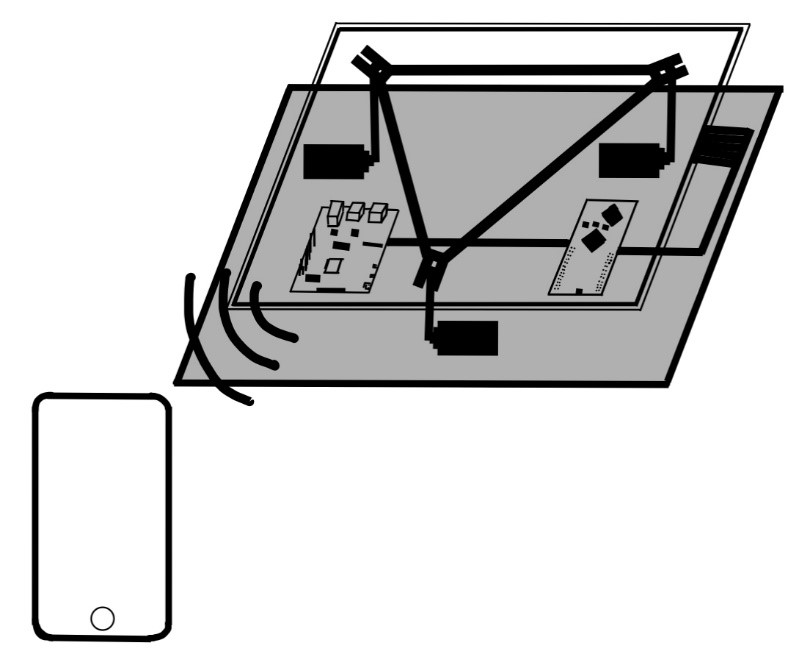
\includegraphics[scale = 0.8]{pics/SkizzeAufbau}
	\caption{Skizzierter Aufbau des Prototypen}
	\label{Skizze}
\end{figure}
In \ref{Skizze} ist eine Skizze des physischen Aufbaus aus dem Lastenheft zum Start des Projektes zu 
sehen. Dabei wurde lediglich graphisch eine mögliche Vorversion des späteren Prototyps gezeichnet. 
\begin{figure}[htbp]
	\centering
	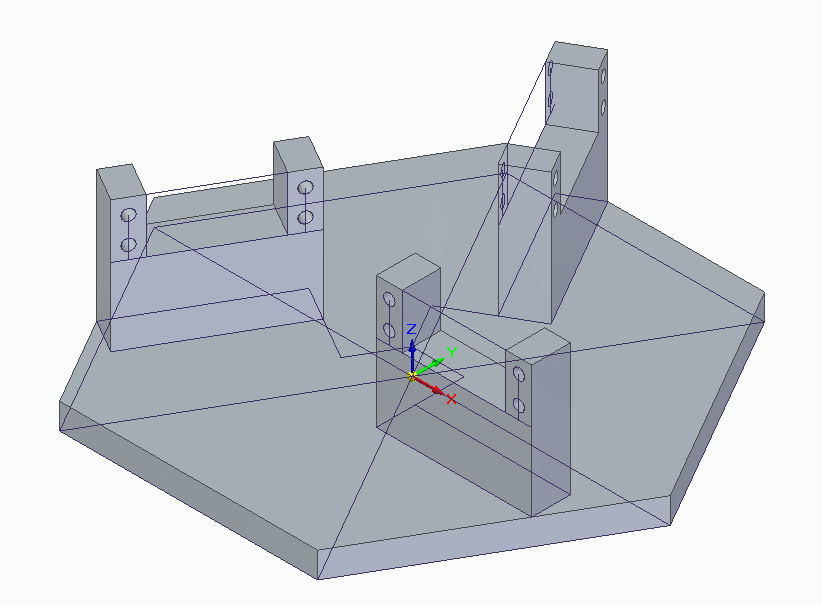
\includegraphics[scale = 0.5]{pics/BildGrundplatte}
	\caption{Grundplatte des Prototypen}
	\label{Grundplatte}
\end{figure}
Im Gegensatz zu \ref{Skizze} wurde eine sechseckige Grundplatte mit den Halterungen für die drei 
Servomotoren mittels Solid Edge 2020 konstruiert und mittels eines 3D-Druckers gefertigt. Diese ist 
in \ref{Grundplatte} zu sehen

Der Druck der Grundplatte dauerte dabei etwa zehn Stunden, was unter anderem an den Ausmaßen der Platte 
(Durchmesser von 20 cm) liegt. Nachdem die Servomotoren in den Halterungen befestigt wurden, hat man die 
Servo-Hebel und Gabelköpfen verbunden, dazu wurden die Servo-Hebel aufgebohrt. Nach dem Zusammenbau hat man 
festgestellt, dass zwischen den Hebeln und dem Gabelkopf noch zu viel Spielraum war, der die Regelung 
beeinträchtigen könnte. Deshalb wurden Unterlegescheiben zur Verringerung des Spiels eingesetzt. Die 
Verbindung zur Platte wird über ein Dreieckskonstrukt \ref{Dreiecksverbindung}, das ebenfalls aus dem 
3D-Drucker kam, hergestellt. 
\begin{figure}[htbp]
	\centering
	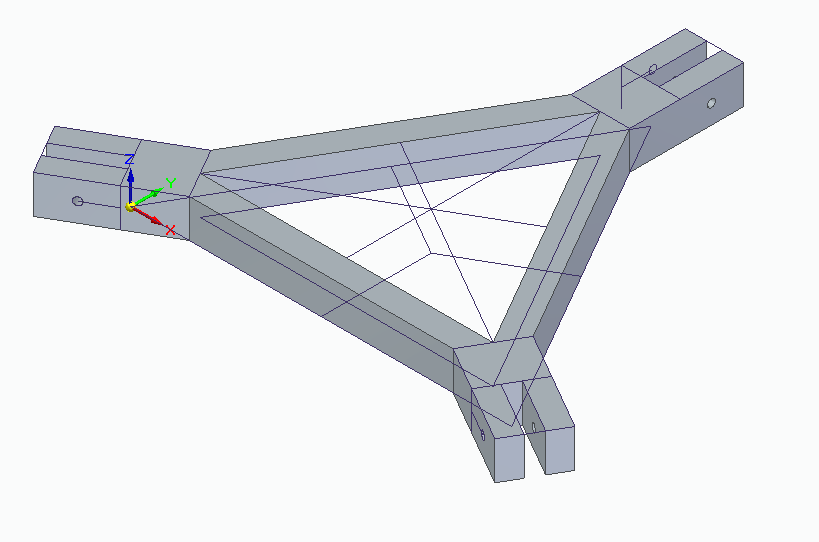
\includegraphics[scale = 0.5]{pics/BildDreieck}
	\caption{Dreiecksverbindung zur Touch-Folie}
	\label{Dreiecksverbindung}
\end{figure}
Dabei war vor allem die korrekte Länge zum Mittelpunkt des Dreiecks, 
respektive der Grundplatte, eine wichtige Größe, da eine falsche Länge nicht mehr die senkrechte 
Ausrichtung des Gabelkopfes zu der Grundplatte zur Folge gehabt hätte. Außerdem mussten die Kugellager 
passend in den Gabelkopf der Dreiecksverbindung eingefügt werden, um eine seitliche Drehung dieser zu 
verhindern.
Der 3D-Druck dieser Verbindung dauerte in etwa sechs Stunden. Die Konstruktion dieser beiden Bauteile 
nahm in etwa fünfzehn Stunden in Anspruch. Diese Dreieckskonstruktion liegt genau über dem markierten 
Dreieck der Grundplatte. Die Touch-Folie befindet sich dabei auf einer Plexiglasplatte, welche mittels 
Silikon mit der Dreiecksverbindung zusammengefügt wurde.
Außerdem wurden vor dem Zusammenbau der Servomotoren mit den Servo-Hebeln, alle Servomotoren in die 
Neutralstellung gesetzt (vgl. PWM-Signale), um die Regelung ebenfalls von einem neutralen Punkt aus zu 
starten. Dabei traten motorspezifische Unterschiede auf die mittels der PWM-Werte ausgeglichen werden 
müssen.Bei der Verkabelung wurden sowohl der XMC und die drei Servomotoren mittels eines gelöteten 
Teilstücks an die gleiche Masse gelegt. Auch die Betriebsspannung der Motoren wurde so gehandhabt.
Zum Fazit:
Die Teile aus dem 3D-Drucker waren insgesamt zufriedenstellend, lediglich die Löcher für die Schrauben 
an der Dreiecksverbindung mussten nachträglich aufgebohrt werden und an einem Gabelkopf der 
Dreiecksverbindung blieben Teile an der Grundplatte des Druckers hängen. Glücklicherweise waren die 
Servomotoren ausreichend stark um die Platte ohne Probleme zu bewegen.

% ----------------------------------------------------------------------------------
% Kapitel 2.2: Software-Architektur
% ----------------------------------------------------------------------------------
\subsection{Software-Architektur}

% ----------------------------------------------------------------------------------
% Kapitel 2.3: Touch-Folie
% ----------------------------------------------------------------------------------
\subsection{Touch-Folie}
\textit{Von Korbinian Federholzner und Philipp Kramer}\newline
\subsubsection{Funktion der Touch Folie}

\begin{figure}[htbp]
	\centering
	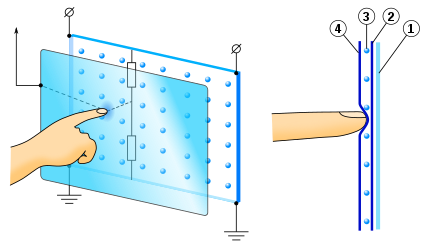
\includegraphics[scale = 0.6]{pics/TouchScreen_5wires.png}
	\caption{Funktion des Touch Panels} 
	\label{fig:TouchPanelFunction}
\end{figure}

Zum Auslesen der Sensorwerte wird ein 5-Wire Rezessives Touchpanael verwendet.
Die Variante mit 5 Kabeln hat den Vorteil, dass für das Auslesen ein 5tes Kabel verwendet wird, welches
ein Analoges Signal liefert. Prinzipiell ist das Panel ein Spannungsteiler, bei \ref{fig:TouchPanelFunction} 
sieht man dass es zwei Schichten hat, welche durch Druck zusammengefügt werden, dadurch ergibt sich 
immer ein anderer Wiederstand je nach dem auf welcher Position man sich auf dem Panel befindet. Der Analoge 
Spannungswert ist also durch diesen Spannungsteiler bestimmt. Damit Sich die Beiden Folien berühren können
muss ein Mindestruck von $1.00 Newton$ gegeben sein. Im Bild \ref{fig:TouchPanelFunction} sieht man dass auf der 
Oberen Seite Spannung und der unteren Masse anliegt. Mit dieser Konstellation kann man nur eine Richtung messen 
also z.B. die X-Koordinate. Um nun auch die Y-Koordinate messen zu können müssen die Pins so umgeschalten werden, 
dass Auf der Linken Seite Spannung und auf der Rechten Seite Masse anliegt. Dadurch ändert wird der Wiederstand der
anderen Seite nun als Spannungsteiler gemessen. 

\subsubsection{Implementierung}
Dadurch, dass die Pins umgeschaltet werden müssen, wurden die GPIO Pins des XMC verwendet. Da das Panel nur mit einer
Frequenz von 50 Hz geschalten werden kann, wurde ein Timer Interrupt definiert. Dieses Interrupt wurde alle 20 ms 
Ausgelöst. Die Interrupt Service Routine startet dann die Messung für den Analog Digital Converter. 
Der Analoge Pin des Panels ist an einem Analog fähigen Pin des XMCs angeschlossen, von welchem mittels des ADCs 
gemessen wird. Der ADC löst sobald er mit dem Messen fertig ist auch eine Interrupt Service Routine aus, in dieser 
wird der gemessene Wert gespeichert und dann die GPIO Pins umgeschalten damit die andere Koordinate gemessen werden kann.
Sind beide Werte vorhanden, so werden die beiden Daten in einem UART Frame verpackt und dann ein UART-Transmit ausgelöst.

\begin{figure}[htbp]
	\centering
	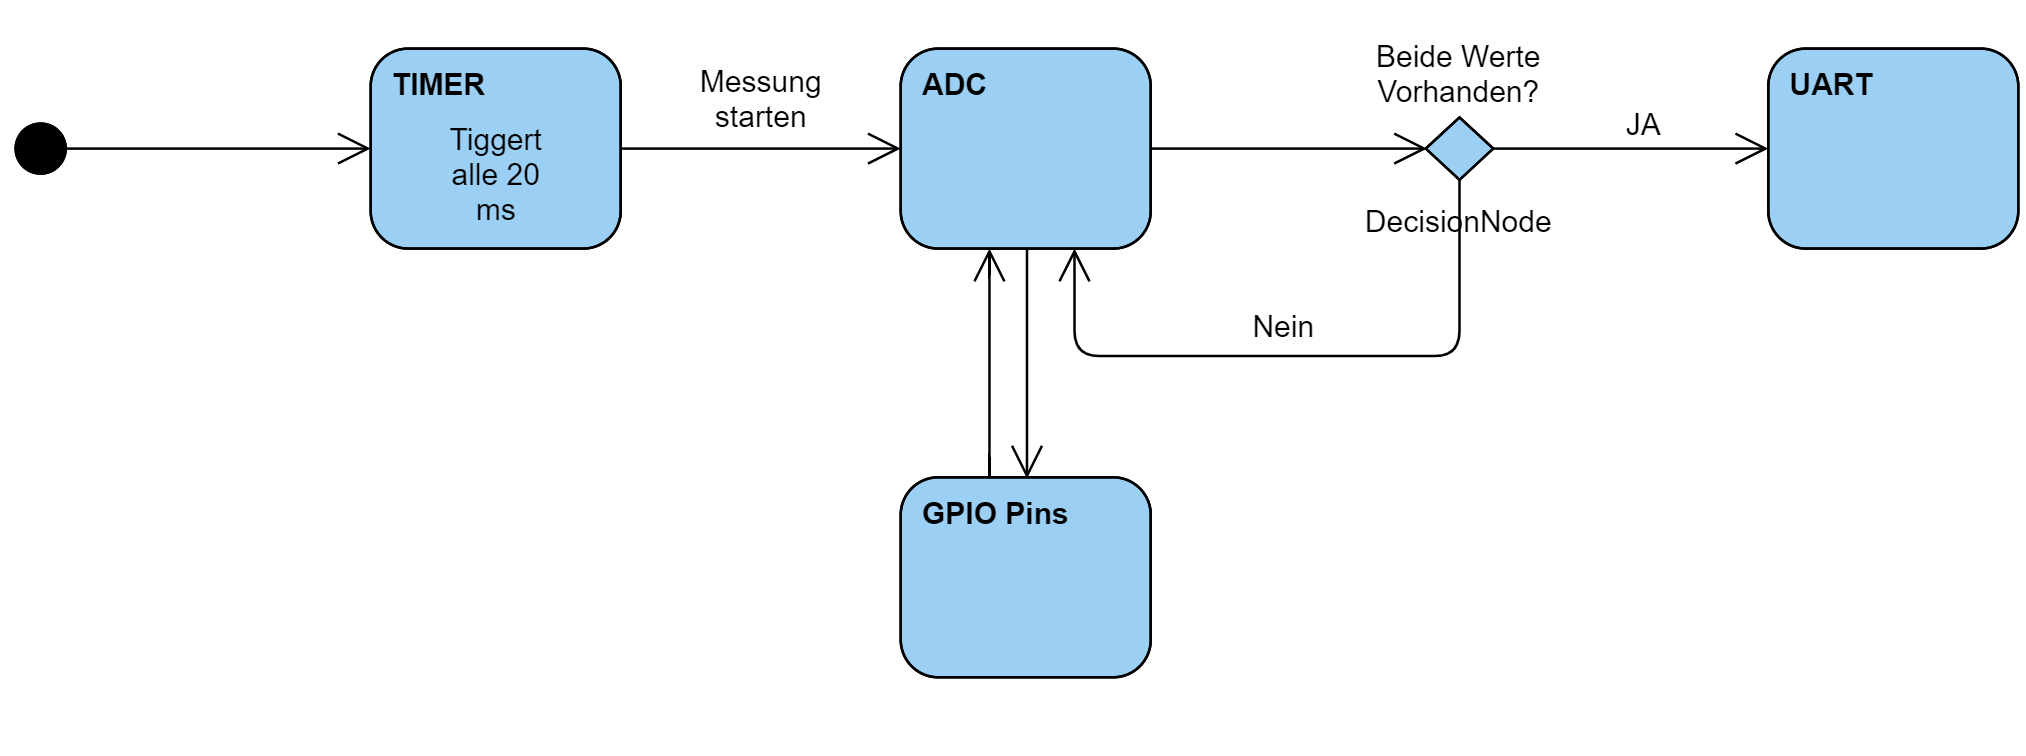
\includegraphics[scale = 0.6]{pics/TouchUML.png}
	\caption{UML Activity Diagramm, der Interrupts}
	\label{TouchUML}
\end{figure}

\subsubsection{Probleme}
Ein Problem im Zuge der Implementierung der Touch-Platte, war die Funktion der ADC-App im Dave4, da bei diesem
keine gute Dokumentation vorhanden war, so war es z.B. schwer herrauszufinden wie die Funktion zum starten der ADC Messung 
hieß. Ein görßeres Problem war der Messfehler des Touch Panels, bei welchem die Platte einen Spannungsabfall je nach Pin hatte.
Bsp: Falls man der X-Achse entlang messen wollte und dabei einen Konstaten Y-Wert beibehielt, so wäre das Erwartete Verhalten,
dass der X-Wert gleich bleiben würde. Jedoch stieg der Wert bei messen entlag der X-Achse konstant an, das selbe war auch auf
der Y-Achse. Um das dieses verhalten der Pins zu eleminieren, wurde versucht das Ganze mittels einer H-Brücke zu lösen, 
jedoch war hier das selbe Problem, über der H-Brücke fiel auch Spannung ab, da 2 Pins immer fest waren und nur 2 Pins
über die Brücke geschalten waren, gab es wieder ein ähnliches Szenario. Die nächste Überlegung, war die Verwendung von Relais.
Leider sind Relais die schnell genug Schalten können relativ Teuer und diese haben einen höheren Verschleiß.
Die Lösung des Problems war, Wiederstände zwischen die Pins des XMCs und der Platte zu schalten. Diese Wiederstände 
minimieren den Fehler, dadruch war der Fehler vernachlässigbar und konnte durch den Regeler ausgeglichen werden. 

\subsection{Programmierung Raspberry Pi}

% ----------------------------------------------------------------------------------
% Kapitel 2.4: UART Schnittstelle
% ----------------------------------------------------------------------------------
\subsection{UART Schnittstelle}
\textit{Von Korbinian Federholzner und Michael Schmidt}\newline
\subsubsection{Funktion}
\begin{figure}[htbp]
	\centering
	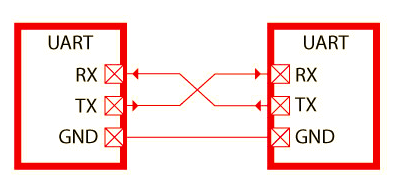
\includegraphics[scale = 0.6]{pics/BildUart1}
	\caption{Grundaufbau der UART-Verbindung}bilder 
	\label{UART}
\end{figure}
Zur Datenübertragung zwischen dem Raspberry Pi und dem XMC Mikrocontroller wurde das Universal 
Asynchronous Receiver Transmitter-Protokoll (UART) verwendet. Dieses ist für schnelle Bitübertragungsraten, 
in unserem Fall eine Baud-Rate von 19200 (Bits pro Sekunde), über eine einzelne Leitung verantwortlich. 
In unserem Fall ist die Übertragung im Modus Full-Duplex und erfordert somit zwei Leitungen, die sich 
kreuzen \ref{UART}.

Grundsätzlich erfolgt die Datenübertragung aufgrund der Einfachheit in Strings, welche jeweils nach dem 
Empfang dekodiert werden. Dabei enthält ein UART-Paket genau ein Zeichen der Zeichenfolge. Ein solches 
Beispielpaket ist in \ref{fig:UARTFrame} zu sehen.Die Übertragung erfolgt dabei auf dem Raspberry Pi über 
die General Purpose In/Out Pins 14 und 15. Dabei ist der Pin 14 der Sender und der Pin 15 der Empfänger 
von den Nachrichten des XMC. Auf dem XMC ist die Pinbelegung variabel und somit flexibler im Gegensatz 
zum Raspberry Pi. Hier wurden die beiden Pins 1.4 und 1.5 gewählt. Hier fungiert Pin 1.5 als Sender und 
Pin 1.4 als Empfänger. Zum Testen wurde vom Raspberry Pi ein vordefinierter String, in diesem Fall 
"`\$123456789!",, an den XMC gesendet. Dieser liest die ankommenden Daten und sendet sie zurück an den 
Raspberry Pi, welcher sie auf dem Bildschirm ausgibt. Dadurch ließen sich die nachfolgenden Fehler in 
der Implementierung und Datenverarbeitung des XMC besser nachvollziehen. Am Anfang des Projektes traten diverse Schwierigkeiten 
beim Testen der Implementierung auf. Zum Beispiel war das Flashen des Programmes auf den XMC unmöglich, 
da ein Fehler generiert wurde, da keine Verbindung zu dem auf dem XMC integrierten Debugger hergestellt 
werden konnte. Nach einem Test mit einem anderem XMC gleicher Bauart wurde festgestellt, dass unser erster 
XMC lediglich defekt war. Nach einem Tausch des verwendeten XMC konnte die Programmierung wieder 
fortfahren, allerdings wurden durch diesen Fehler insgesamt ca. 10 Stunden Arbeitszeit in die Fehlersuche 
investiert. Dieses Problem behinderte auch das Arbeitspaket "`PWM-Signale".
Ein weiteres Problem, auf das wir gestoßen sind, war ein Fehler in der Interrupt-Funktion. Auf dem XMC 
lassen sich unter Dave4 in den zur Verfügung gestellten APPs diverse Empfangs- und Sendeoptionen festlegen. 
Darunter war auch das Empfangen mittels eines Interrupts. Dieses Interrupt wurde jedoch beim Testen nicht 
aufgerufen und somit die ankommenden Daten nicht aus dem Speicher ausgelesen. Um dieses Problem zu umgehen 
wurde mittels der Dave4-APP NVIC/Interrupt ein Hardwareinterrupt konfiguriert, welches bei einer Änderung 
des Buses von logisch 0 auf logisch 1 ausgelöst wird und die ankommenden Daten verarbeitet. Dabei traten 
jedoch weitere Probleme auf, wie z.B. die ankommenden Daten waren nicht vollständig, da das Interrupt zu 
schnell ausgelöst wurde und die verbleibenden Daten nicht in den Buffer geschrieben wurden, oder das erste 
Zeichen wurden als "`0" \,interpretiert. Dies hatte folgenden Grund: Das Interrupt wurde zu langsam geöffnet 
und im Buffer kam es zu einem Overflow, sodass die ersten Werte bereits wieder mit "`0"\, überschrieben wurde, 
welche das UART-Protokoll als Byte-Stream-Ende interpretiert und somit nicht korrekte Daten liefert.
Nach intensiver Suche in der integrierten Dokumentation in Dave 4, welche jedoch erst nach einigem Suchen 
gefunden wurde, stießen wir auf eine Funktion:\, "`UART\_StartRecieveIRQ"\,, deren Implementierung anscheinend 
erforderlich war, um mittels der in der UART-APP vorprogrammierten Interrupt-Option die ankommenden Daten 
auszulesen %\cite {infineonforums}
. Diese Funktion setzt einen Interrupt-Request und muss 
kontinuierlich nach dem erstmaligen Empfangen ausgeführt werden, um eine fehlerfreie Abarbeitung zu 
gewährleisten. Somit wird sie nach jedem Empfangsvorgang auf dem XMC in der Interrupt-Routine neu 
aufgerufen.


% ----------------------------------------------------------------------------------
% Kapitel 2.5: Datenübertragungsformate
% ----------------------------------------------------------------------------------
\subsubsection{Datenübertragungsformate}
\textit{Von Korbinian Federholzner und Michael Schmidt}\newline
Um eine eindeutige Übertragung zu gewährleisten, wurde sich auf ein standardisiertes Format festgelegt. 
Dabei wurden eine bestimmte Anzahl Pakete in einer bestimmten Reihenfolge gesendet, wobei pro Paket immer 
ein Zeichen des Strings übertragen wird, wie in \ref{fig:UARTFrame}verdeutlicht wird.
\begin{figure}[htbp]
	\centering
	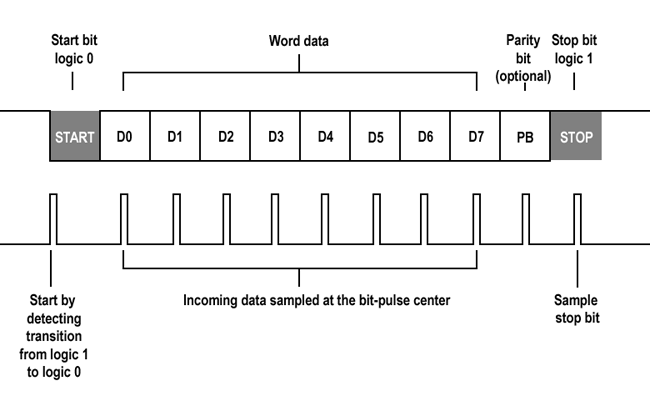
\includegraphics[scale = 0.44]{pics/Uartframe}
	\caption{Aufbau eines UART-Frames\cite {electricimp}}
	\label{UARTFrame}
\end{figure}
Diese Zeichen werden dann aneinandergereiht und ergeben die unten beschriebenen Formate. Dabei hat die 
Kommunikation, bei der der Raspberry Pi der Sender und der XMC 4500 der Empfänger ist folgendes Format 
\ref{UART Servo}.
\begin{figure}[htbp]
	\centering
	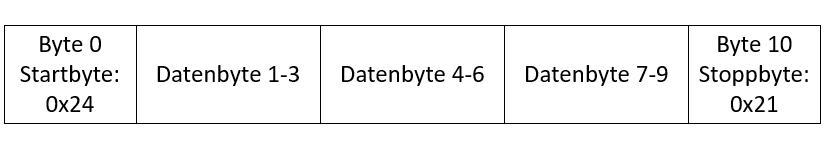
\includegraphics[scale = 0.44]{pics/Uartservo}
	\caption{Aufbau eines Datenpakets mit Servowerten}
	\label{UART Servo}
\end{figure}
Übertragen werden hierbei die aktuellen Werte für die PWM-Signalgenerierung, deren Werte sich zwischen 
450 und 1050 befinden. Dies ist durch die maximale Auslenkung der Servomotoren begründet. Um weitere Bytes 
zu sparen wird nur der Offset von dem Grundwert 450 übermittelt. Dieser wird in einer nachfolgenden 
Funktion wieder dekodiert und in die jeweiligen Variablen gespeichert, auf die die PWM-Signalgenerierung 
zugreift. Dabei befinden sich in den ersten drei Zeichen des Datenteils (Byte 1-3) die Werte für den ersten 
Servomotor., in den zweiten drei (Byte 4-6) die Werte für den zweiten Servomotor und in den letzten drei 
(Byte 6-9) die Werte für den dritten Servomotor, wie in der Abbildung 6 dargestellt. Das Startbyte 0, 
"`0x24"\, und das Stoppbyte 10 "`0x21"\, dienen dabei der Erkennung der feststehenden Feldlänge, um eine korrekte 
und vollständige Übermittlung zu gewährleisten. Die Kommunikation zwischen XMC 4500 und dem Raspberry Pi 
erfolgt über mehrere Formate, da wir mehrere unterschiedliche Nachrichten auf dem Raspberry Pi verarbeiten 
müssen. Zum einen wären da die Übertragung der X- und Y-Koordinaten der Touch-Folie und zum anderen die 
Rückgabewerte der Potentiometer aus den Servomotoren. Um zwischen den beiden Nachrichtentypen, die 
unterschiedliche Längen und Formate haben zu unterscheiden haben wir eine Nachrichten-Identifikationsnummer 
(Message-ID) eingeführt, welche vor den jeweiligen Dekodierungsfunktionen überprüft wird. Lediglich der 
Datenteil unterscheidet sich zwischen den beiden Typen. Da sie als String übertragen werden, ist das 
System problemlos auf bis zu 100 unterschiedliche Nachrichtenformate erweiterbar. Um das bestehende System 
zu erweitern muss lediglich eine zugehörige Dekodierungsfunktion auf dem Raspberry Pi programmiert werden 
und ein korrekter Sendevorgang auf dem XMC sichergestellt werden. Die Nachricht mit den Werten der 
Touch-Folie hat die Message-ID "`00" \,und wird wie folgt übertragen \ref{UART Platte}.
\begin{figure}[htbp]
	\centering
	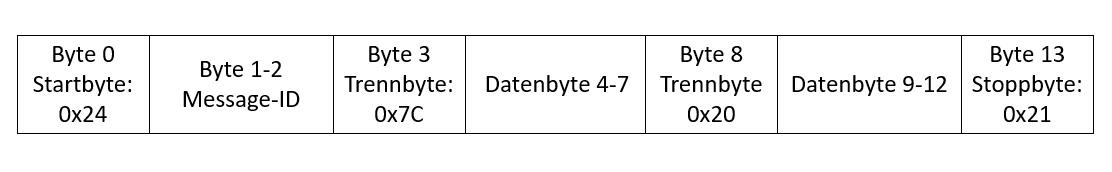
\includegraphics[scale = 0.44]{pics/Uartplatte}
	\caption{Aufbau eines Datenpakets mit den Werten der Touch-Folie}
	\label{UART Platte}
\end{figure}
Auch hier sind Start und Ende der Nachricht wieder mit einem Zeichen, zum Erkennen der korrekten 
Feldlänge, markiert. Dabei werden die Werte der Touch-Folie, die bereits in X-, bzw. Y-Koordinaten 
umgerechnet wurden übertragen. Diese sind in den Datenbytes 4-7 (X-Koordinate) und Datenbytes 9-12 
(Y-Koordinate) kodiert. Zwischen den einzelnen Koordinatenwerten und der Message-ID wurde noch ein 
Trennbyte eingeführt, da die Koordinaten unterschiedliche Länge haben können (3 oder 4 Zeichen). Auf dem 
Raspberry Pi werden diese wieder in integer-Werte umgerechnet und als Koordinaten an die Regelung 
übergeben.

\subsubsection{CRC-Check}
Da der Austausch der mit UART immer wieder Bit-Errors hatte, gab es immer wieder Störungen an den Servos.
Um die Bitfehler zu erkennen wurde ein CRC-Check implementiert, welcher ein Generatorpolynom über das
gesamte Packet ermittelt. Für die Implementierung wurde eine CRC-Tabelle benutzt, da diese den Vorteil hat,
dass der CRC-Betrag nicht komplett berechnet werden muss, sondern nur ein Teil. Über diesen Anteil kann 
der Wert in der Tabelle nachgeschlagen werden und dieser als CRC-Wert verwendet werden. Der Vorteil einer solchen
Tabelle ist die Performance, da die komplette Rechnung aufwändiger wäre und mehr Performance ziehen würde. Der CRC-Check ist momemtan nur in
der Richtung vom XMC zum Raspberry Pi implementiert, da nur dort die Bit-Errors auftraten. Vom Touchpanel des XMCs zum PI wurde nicht unbedingt ein CRC benötigt,
da auf dem PI ein Kalman-Filter davorgeschalten wurde der diese Fehler ausgleicht. 
Der CRC könnte hier in Zukunft noch implementiert werden.

\subsubsection{Probleme}
Die größten Probleme beim UART war die Dave4 Dokumentation des XMCs. Online findet man ein sehr detailiertes Handbuch zum 
XMC4500, jedoch nahezu keine Dokumentation wie die enthaltenen Dave4 Apps funktionieren. Die OTH Rechner haben bei der Dave4 IDE keine 
Help Manuals, was das Ganze noch erschwert. Die Lösung dieses Problems war, die Help Manuals auf Dave4 manuell 
nachzuinstallieren. In diesem git es sehr viele nützliche Informationen wie UART eigentlich mittels der App funktioniert und welche Bedeutung die Funktionen genau haben.

\subsubsection{Ausbick}
Folgende Punkte waren aufgrund von Zeitmangel nicht mehr funktionsfähig zu implementieren.
Der CRC-Check ist momentan aus zeitlichen Gründen in nur eine Richtung implementiert. Es ist zwar nicht wegen des Kalman-Filters nicht unbedingt nötig,aber
 es wäre trozdem nicht schlecht in Richtung vom XMC zum PI einen CRC-Check zu haben. 
Auf dem Branch XMC/HDLCframing ist eine Version des UART Frames die sich an dem HDLC Format orientiert. Diese 
ist warscheinlich stabiler als die momentane. Der Code auf dem Branch ist so gut wie fertig, jedoch war das Framing welches 
in der Endversion ist, schon gut genug getestet, sodass dieser ungetestet Code nicht nötig war.
% ----------------------------------------------------------------------------------
% Kapitel 2.6: Reglerentwicklung
% ----------------------------------------------------------------------------------
\subsection{Reglerentwicklung}
\textit{Von Michael Braun und Philipp Kramer}\newline

% ----------------------------------------------------------------------------------
% Kapitel 2.7: PWM Signale
% ----------------------------------------------------------------------------------
\subsection{PWM-Signale}
\textit{Von Michael Braun und Michael Schmidt}\newline

Die Ansteuerung der Servomotoren erfolgt über ein 50 Hz PWM-Signal, welches mittels der Funktion 
"`PWM\_SetDutyCycle"\, auf die jeweils aktuellen Werte geändert wird. Diese Funktion wandelt automatisch 
die Werte die im Promillebereich, im Format $0-10000$, angegeben werden, in die richtige Länge des 
Hochanteils des PWM-Signals um. Diese Funktionen werden von den Dave 4- eigenen APPs zu Verfügung 
gestellt. Dabei sind durch die Servomotoren einige Werte vorgegeben \ref {servowerte}.

\begin{tabularx}{\textwidth}{p{0.25\textwidth}|X|X|X|X|X|}
\hline
 Bezeichnung 		& Wert in ms (zu 20ms/50Hz) & Wert in Prozent 	& Wert in Promille \\
\hline
 Minimalstellung		& 0,9						& 4,5				& 450 \\
\hline
 Neutralstellung		& 1,5						& 7,5				& 750 \\
\hline
 Maximalstellung		&2,1						& 10,5				& 1050\\
\hline
%\caption{Tabelle: Werte der Servomotoren}
%\label{tbl:servowerte}
\end{tabularx}

Sollten die übertragenen Werte den Maximalwert von 1050 überschreiten, werden sie lediglich auf den 
Maximalwert gesetzt, um eine korrekte Ansteuerung der Servomotoren zu gewährleisten. Diese Werte werden 
kontinuierlich von der Regelung verändert und über die Pins 3.0, 3.3 und 3.4 des XMC an die Servomotoren 
ausgegeben. Dies wird in einem Interrupt abgearbeitet, das im 50 Hz Takt aufgerufen wird. Dabei sind jedoch 
noch motorenspezifische Unterschiede aufgetreten, die in Tabelle 3 aufgeführt werde. Diese sind nötig, um 
die Platte initial in eine ebene Nullstellung zu positionieren.

\begin{tabularx}{4cm}{|l|l|}
\hline
 Servomotor		& Offset \\
\hline
 1				& 35	\\
\hline
 2				& 15\\
\hline
 3				& 5	\\
\hline
%\caption{Tabelle: Werte der Servomotoren}
%\label{tbl:offsets}
\end{tabularx}


%TODO
Außerdem wird die Auslenkung der Hebel durch die Aufhängung der Motoren begrenzt, da ab einem 
bestimmten Wert die Platte an diese stößt. Dadurch ergeben sich folgende Einschränkungen:
Einschränkungen messen


Abgesehen von Anfangsschwierigkeiten mit dem Flashen des XMCs, war die Ansteuerung über PWM-Signale 
mit den internen Dave 4 APPs sehr einfach zu lösen, lediglich die Berechnung der Einschränkungen und 
die korrekte Übergabe der Werte stellten eine kleine Herausforderung dar.

% ----------------------------------------------------------------------------------
% Kapitel 2.8: Threading auf dem Raspberry Pi
% ----------------------------------------------------------------------------------
\subsection{Threading auf dem Raspberry}
\textit{Von Korbinian Federholzner}\newline
Das erhalten der UDP-Packete und der UART-Frames, wurde in Blocking-Loops implementiert, dadurch wäre die Anwendung 
die ganze Zeit durch diese Loops blockiert. Um dieses Verhalten zu umgehen wurden alle Listening-Loops in eigene Threads
verschoben. Da die Anwendung zentral von einem Button gesteuert wird, welcher zwischen den Modus zum Regeln und dem 
Modus zur manuelle Steuerung mit der App wechselt, gesteuert wird, befindet sich die Ansteuerung des Buttons im main Thread.
Für den Regeler und das manuelle Ansteuern gibt es auch wieder zwei Threads welche je nach Zustand des Buttons auf 
aktiv gesetzt werden. Um den Zugriff auf die gelesenen Daten von UART und UDP sicher zu gewährleisten, wurde mittels 
Mutex der Zugriff auf die Daten abgesichert. Dabei kann nur entweder UART schreiben oder der Benutzer die Daten abfragen,
niemals beide gleichzeitig.


% ----------------------------------------------------------------------------------
% Kapitel 2.9: UDP-Socket
% ----------------------------------------------------------------------------------
\subsection{UDP-Socket}
\textit{Von Patrick Lesch}\newline

% ----------------------------------------------------------------------------------
% Kapitel 2.10: IOS-Appliaktion
% ----------------------------------------------------------------------------------
\subsection{iOS-Applikation}
\textit{Von Patrick Lesch}\newline


% ----------------------------------------------------------------------------------
% Kapitel 2.11: Zusammenführung
% ----------------------------------------------------------------------------------
\subsection{Zusammenführung der einzelnen Komponenten}
Diverse Probleme gab es beim Merge-Vorgang auf Gitlab mit den durch Dave4 automatisch erstellten Files. 
Diese erfassen die konfigurierten Einstellungen der XMC APPs und überführen diese in ausführbaren Code. 
Dieses Problem wurde dadurch gelöst, dass man die Einstellungen auf einem Branch durchgeführt hat und 
lediglich die selbstgeschriebenen Code-Files zusammengeführt hat.

\pagebreak
% ----------------------------------------------------------------------------------
% Kapitel 3: Benutzerhandbuch
% ----------------------------------------------------------------------------------
\section{Benutzerhandbuch}


\pagebreak
% ----------------------------------------------------------------------------------
% Kapitel 4: Fazit/Zusammenfassung
% ----------------------------------------------------------------------------------
\section{Fazit}

% ----------------------------------------------------------------------------------
% Kleine Einführung in LaTeX-Elemente
% ----------------------------------------------------------------------------------
%\section{\LaTeX-Elemente}
%Dieser Abschnitt beinhaltet lediglich einige Informationen über \LaTeX-Distributionen, Editoren und \LaTeX-Elemente, die Ihnen beim Einstieg in das \LaTeX-Textsatzsystem helfen sollen.

%\subsection{\LaTeX-Distributionen nach Betriebssystemen}

%\subsubsection{\LaTeX-Distributionen}
%Folgende Haupt-\LaTeX-Distributionen stehen Ihnen zur Verfügung:
%\begin{itemize}
%  \item Windows:\quad \texttt{MiKTeX}\quad Webseite:\quad\url{http://www.miktex.org}
%  \item Linux/Unix:\quad \texttt{TeX Live}\quad Webseite:\quad\url{http://tug.org/texlive/}
%  \item Mac OS:\quad \texttt{MacTeX}\quad Webseite:\quad\url{http://www.tug.org/mactex/}
%\end{itemize}

%\subsubsection{\LaTeX-Editoren}
%Auf folgenden Webseiten können Sie einige hilfreiche \LaTeX-Editoren finden:
%\begin{itemize}
%  \item Windows/Linux/Mac OS: \url{http://www.xm1math.net/texmaker/}
%  \item Windiws: \url{http://www.texniccenter.org/}
%  \item Mac OS: \url{http://pages.uoregon.edu/koch/texshop/}
%\end{itemize}

%Falls bei den oben genannten Editoren kein passender vorhanden war, findet sich auf Wikipedia eine Zusammenstellung vieler weiterer \LaTeX-Editoren:\\
%\url{https://en.wikipedia.org/wiki/Comparison_of_TeX_editors}

%Für die PDF-Anzeige empfiehlt sich SumatraPDF: \\ 
%\url{https://www.sumatrapdfreader.org/free-pdf-reader.html}.


%\subsection{Bilder}
%Zum Einfügen eines Bildes, siehe Abbildung \ref{fig:reversi01}, werden die \texttt{minipage}-Umgebung und der Befehl \texttt{$\backslash$includegraphics} genutzt, da die Bilder so gut positioniert und einfach integriert und skaliert werden können.

%\vspace{1em}
%\begin{minipage}{\linewidth}
%	\centering
%	\includegraphics[width=0.5\linewidth]{pics/gamefield01.png}
%	\captionof{figure}[Spielfeld 01]{Unbespieltes Spielfeld}
%	\label{fig:reversi01}
%\end{minipage}


%Nachdem das Spielt gestartet wurde und beide Spielphasen durchlaufen wurden, siegt schließlich der Spieler mit der Farbe rot.

%\vspace{1em}
%\begin{minipage}{\linewidth}
%	\centering
%	\includegraphics[width=0.5\linewidth]{pics/gamefield02.png}
%	\captionof{figure}[Spielfeld 02]{Finales Spielfeld}
%	\label{fig:reversi2}
%\end{minipage}


%\subsection{Tabellen}
%In diesem Abschnitt wird eine Tabelle (siehe Tabelle \ref{tab:beispiel}) dargestellt.

%\vspace{1em}
%\begin{table}[!h]
%	\centering
%	\begin{tabular}{|l|l|l|}
%		\hline
%		\textbf{Name} & \textbf{Name} & \textbf{Name}\\
%		\hline
%		1 & 2 & 3\\
%		\hline
%		4 & 5 & 6\\
%		\hline
%		7 & 8 & 9\\
%		\hline
%	\end{tabular}
%	\caption{Beispieltabelle}
%	\label{tab:beispiel}
%\end{table}


%\subsection{Auflistung}
%Für Auflistungen wird die \texttt{enumerate}- oder \texttt{itemize}-Umgebung genutzt.

%\begin{itemize}
%	\item Nur
%	\item ein
%	\item Beispiel.
%\end{itemize}

%\subsection{Listings}
%Sehen Sie in Listing \ref{lst:helloworld} ein Beispiel für das Einbinden von Quellcode mit Syntax-Highlighting.

%\vspace{1em}
%\lstinputlisting[caption=Brute Force-Ansatz für das MaxTeilsum2D-Problem, label=lst:maxTeilsumZweiD,basicstyle=\ttfamily\scriptsize]{code/maxTeilsum2DBruteForce.txt}
%\lstinputlisting[caption=Hello World Program, label=lst:helloworld,basicstyle=\ttfamily\scriptsize]{code/helloworld.c}

%\subsection{Gleichungen}
%Formatierung von Formeln:
%\begin{itemize}
%  \item Formelzeichen sind in kursiv zu setzen
%  \item Zahlen, Einheiten und Funktionsnamen sind in normaler Schriftart zu setzen (nicht kursiv)
%  \item Häufig wird fälschlicherweise das Symbol * als Multiplikationszeichen verwendet
%  \item Zwischen Zahl und Einheit ist ein Leerzeichen zu setzen
%\end{itemize}

%Frequency Modulation (FM) is a wireless transmission system patent-registered by Edwin H. Armstrong in 1933. It is still widespread in the area of audio broadcasting today. In case of the frequency modulation the amplitude of the desired message signal varies the frequency (the argument) of the sinusoidal carrier. The general FM oscillation is formulated with 
%\begin{equation}
%u_{\textrm{FM}}(t)= a_0 \cos(\Psi(t)+\varphi_0) 
%\label{eqn:fmosc}
%\end{equation}

%To simplify matters, only an one-tone modulation signal is considered to characterize the spectrum of FM-signals at first
%\begin{multline}
%u_{\textrm{FM}}(t)=\hat u_T \cdot [J_0(\eta)\cos\omega_Tt + \sum_{n=1}^{+\infty} J_n(\eta) \cdot (\cos[(\omega_T+n\omega_1)t]+(-1)^n \cos[(\omega_T-n\omega_1)t])] 
%\\ \ \mbox{with Bessel functions:} \ J_n(\eta)= \frac{(-1)^n}{\pi} \int_0^{\pi} e^{j\eta\sin x} \cdot \cos(nx) dx 
%\end{multline}

%\subsection{Verwendung von Abkürzungen}
%Die Abkürzungen können so verwendet werden:
%Beim ersten Mal der Verwendung (vgl. Einleitung) wird die Abkürzung ausgeschrieben \ac{BA}. Beim zweiten Mal oder folgenden Malen wird nur noch die Abkürzung verwendet \ac{BA}.
%Aber setzen Sie Abkürzungen sparsam ein.

%\subsection{Tipps}
%Die Quellen befinden sich in der Datei \textit{quellen.bib}. 
%Alle Literaturangaben müssen im Text referenziert werden. Die höchstwertigen Quellen stellen dabei Zeitschriftenartikel \cite{Laprie2004}, gefolgt von Konferenzbeiträgen \cite{Agrou2011}, Patenten \cite{Grisenthwaite2012}, Standards \cite{ARINC2005}, Fachbüchern \cite{Kopetz2011},  Datenblättern \cite{Freescale2015}, Techreports und White-Papern \cite{Aswadhati2011} und zuletzt Onlinequellen \cite{Xil2010} dar.

\pagebreak



% ----------------------------------------------------------------------------------------------------------
% Anhang
% ----------------------------------------------------------------------------------------------------------
\pagenumbering{Roman}
\setcounter{page}{1}
\lhead{Anhang \thesection}

\begin{appendix}
\section*{Anhang}
\phantomsection
\addcontentsline{toc}{section}{Anhang}
\addtocontents{toc}{\vspace{-0.5em}}

%\section{Domändenmodell}
%Ein toller Anhang.


%\subsection*{Screenshot}
%\label{app:screenshot}
%Unterkategorie, die nicht im Inhaltsverzeichnis auftaucht.
%\pagebreak

\end{appendix}


% ----------------------------------------------------------------------------------------------------------
% Abkürzungsverzeichnis
% ----------------------------------------------------------------------------------------------------------
\section{Abkürzungsverzeichnis}
\begin{acronym}[KDE]
	\acro{BA}[BA]{Bachelorarbeit}
	\acro{MA}[MA]{Masterarbeit}

\end{acronym}
\pagebreak


% ----------------------------------------------------------------------------------------------------------
% Abbildungsverzeichnis (optional)
% ----------------------------------------------------------------------------------------------------------
\section {Abbildungsverzeichnis}
\listoffigures
\pagebreak

% ----------------------------------------------------------------------------------------------------------
% Tabellenverzeichnis (optional)
% ----------------------------------------------------------------------------------------------------------
\listoftables
\pagebreak


% ----------------------------------------------------------------------------------------------------------
% Literatur
% ----------------------------------------------------------------------------------------------------------
\renewcommand\refname{Literaturverzeichnis}
\lhead{}
%\bibliographystyle{alpha}
\bibliographystyle{ieeetr}
\bibliography{quellen}
\pagebreak

\section {Bestelliste}
%\begin{tabularx}{\textwidth}{p{0.25\textwidth}|l|l|l|l|l|X|}
%\hline
% Produktname					& Produkt Nr.			& Kosten				& Stück  &Gesamtkosten &Link \\
%\hline
% Servomotoren	&209913-62 &\euro{25,90} &3 &\euro{77,70}	&https://www.conrad.de/de/p/hitec-standard-servo-hs-5485hb-digital-servo-getriebe-material-karbonite-stecksystem-jr-209913.html \\
%\hline
% Servo-Hebel &1530677-VQ &\euro{6,99} &3 & \euro{20,91} &https://www.conrad.de/de/p/reely-alu-servohebel-geklemmt-47-mm-passend-fuer-futaba-servohebelkranz-anzahl-bohrungen-5-1530677.html \\
%\hline
% Gabelkopf &239186-62 &\euro{7,55} & 3 &\euro{22,65} &https://www.conrad.de/de/p/modelcraft-aluminium-gabelkopf-mit-innengewinde-m3-5-st-239186.html \\
%\hline
% Kugelgelenk &221868-62 &\euro{6,71} &3 &\euro{20,13} &https://www.conrad.de/de/p/modelcraft-stahl-kugelkopf-mit-aussengewinde-m3-1-st-221868.html \\
%\hline
% Bildschirm &1503822-62 &\euro{43,99} &1 &\euro{43,99} &https://www.conrad.de/de/p/joy-it-rb-lcd5-touchscreen-modul-12-7-cm-5-zoll-800-x-480-pixel-passend-fuer-raspberry-pi-inkl-touchpen-1503822.html \\
%\hline
% Touch-Folie &710-5240 &\euro{99,73} &1 &\euro{99,73} &https://de.rs-online.com/web/p/touchscreen-sensoren/7105240/ \\
%\hline
%\hline
% Gesamt: & & & &\euro{285,17} & \\
%\hline
%\caption{Tabelle: Bestellliste}
%\label{tbl:bestellliste}
%\end{tabularx}

\begin{figure}[htbp]
	\centering
	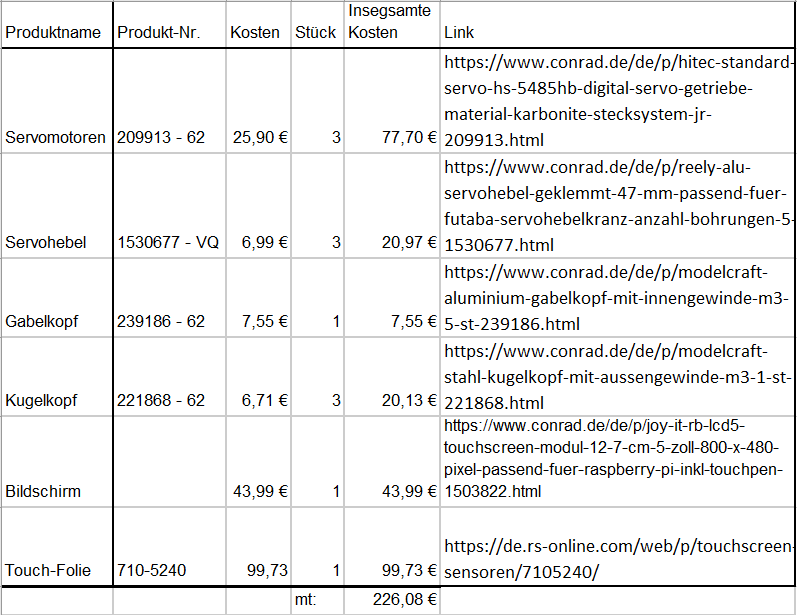
\includegraphics[scale = 0.8]{pics/Bestelliste}
	\caption{Bestellliste und Kosten des Projektes}
	\label{bestell}
\end{figure}


\end{document}
